\begin{figure*}[t]
  \centering
  \begin{subfigure}[t]{0.235\textwidth}
    \centering
    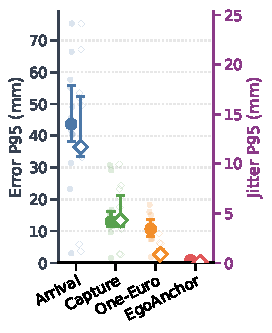
\includegraphics[width=\linewidth]{figures/panels/figure2a_static_translation.pdf}
    \caption{静止平移}
    \label{fig:exp1-static-translation}
  \end{subfigure}\hfill
  \begin{subfigure}[t]{0.235\textwidth}
    \centering
    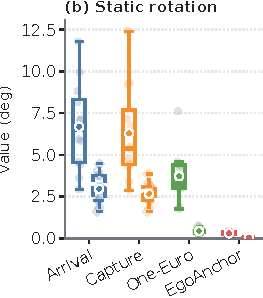
\includegraphics[width=\linewidth]{figures/panels/figure2b_static_rotation.pdf}
    \caption{静止旋转}
    \label{fig:exp1-static-rotation}
  \end{subfigure}\hfill
  \begin{subfigure}[t]{0.235\textwidth}
    \centering
    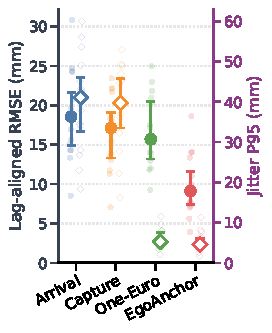
\includegraphics[width=\linewidth]{figures/panels/figure2c_dynamic_translation.pdf}
    \caption{动态平移}
    \label{fig:exp1-dynamic-translation}
  \end{subfigure}\hfill
  \begin{subfigure}[t]{0.235\textwidth}
    \centering
    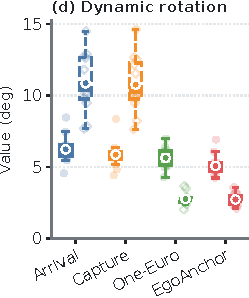
\includegraphics[width=\linewidth]{figures/panels/figure2d_dynamic_rotation.pdf}
    \caption{动态旋转}
    \label{fig:exp1-dynamic-rotation}
  \end{subfigure}
  \caption{实验一的平移与旋转误差--抖动分布。每个方法左移圆点对应左轴误差，右移空心菱形对应右轴抖动；浅色点为片段值，醒目标记与误差条为中位数和 IQR。静止误差采用中心化 P95，动态误差采用 lag-aligned RMSE；动态抖动采用同一最佳时延下残差轨迹的帧间增量 P95，因此不把真实运动计为抖动。左右纵轴相互独立，均为越低越好。}
  \label{fig:exp1-final}
\end{figure*}
